
\section{Background and Related Work}

% In this section, we provide a brief overview of Large Language Models (LLMs), the \LPP project (a framework for LLM inference on edge), and finally look at existing works that enable efficient development of edge accelerators for LLMs.


%*********************************************************************************************

\subsection{Large Language Models }

LLMs are a family of ML models that use the Transformer~\cite{vaswani2017attention} architecture as the key component, and are pre-trained on large amounts of language data.
People usually use them by fine-tuning with downstream task-specific datasets.
LLMs usually have large amounts of parameters.
For example, Llama is designed to start with 7B parameters~\cite{touvron2023llama}.
Also, many types of language-generating LLMs auto-regressively compute the next tokens (chunks of text) by using the previously cached information.
This computation paradigm, called KV cache~\cite{kwon2023efficient}, introduces a large amount of memory overheads while improving performance.

Quantization techniques are extensively employed to deploy parameter-intensive LLMs on resource-constrained edge devices.
For example, utilizing 8-bit quantization facilitates the retention of model accuracy while significantly reducing the model size~\cite{Zafrir2019Q8BERT, Wan2024ASP-DAC}.
In addition, prior studies have demonstrated efforts in experimenting with smaller number of bits, such as 4-bit quantization, to enable the operation of LLMs on edge devices while upholding accuracy levels~\cite{Shen2024EdgeQAT}. 
Another technique that can be considered is block floating point (BFP) quantization, and there have been some works~\cite{Rouhani2023Microscaling} comparing the efficacy of BPF to traditional integer (8/4-bit) quantization.

% In
% \cite{Rouhani2023Microscaling} described the efficacy of block floating point quantization compared to traditional narrow precision quantization.


%*********************************************************************************************

\subsection{Inference framework: \LPP}

\LPP~\cite{LLP} is a pure C/C++ library with minimal external dependencies for enabling LLMs inference on a wide range of hardware.
Currently, \LPP supports a wide range of LLMs, including some multi-modal and custom-defined models.
Additionally, it supports 1.5-bit, 2-bit, 3-bit, 4-bit, 5-bit, 6-bit, and 8-bit BFP quantization.
%In \LPP implementation, BFP quantization is leveraged to quantize the weights of the LLMs, and it includes type 0 and type 1 quantization, typically denoted as \( Q{x\_y} \), where \( x \) represents the number of bits and \( y \) denotes the type of quantization.
In \LPP, BFP quantization is leveraged to quantize the weights of the LLMs, and it includes few quantization variations.
These variations are typically denoted as \( Q{x\_y} \), where \( x \) represents the number of bits per weight and \( y \) denotes the type of quantization.

\LPP~\cite{LLP} employs the GPT-Generated Unified Format model format (GGUF) to represent LLMs.
Within this format, it is possible to represent the weights of an LLM with as few as 1.5 bits using BFP quantization.
These quantized weights enable users to run LLMs on resource-constrained edge devices such as the Raspberry Pi and the Pixel phone~\cite{simonwillison}.

LLM inference is possible on edge devices equipped with CPUs or GPUs due to the optimized support provided by \LPP~\cite{LLP} for AVX, AVX2, and AVX-512 on x86 architectures as well as custom CUDA kernels for running on NVIDIA GPUs.
However, LLM inference on resource-constrained devices, especially on FPGAs is not straightforward, as the design process for new FPGA-based accelerators has not been integrated with inference platforms like \LPP yet.
 

%*********************************************************************************************

\subsection{FPGA-based acceleration for LLMs}

Previous works have described acceleration ideas for running LLMs on FPGAs~\cite{Kachris2024Survey}.
The focus was generally to accelerate LLM inference.
Additionally, they have addressed the challenge of executing a wide variation of LLMs on FPGAs by proposing an overlay FPGA-based processor~\cite{Khan2021NPE}.
However, research has yet to focus on developing design flows and enabling explorations of new FPGA-based acceleration ideas for the latest LLMs.
While transformer accelerator design that commences with the C/C++ code of an LLM exists~\cite{Lu2020Transformer}, their primary focus lies on the accelerator design aspect, not necessarily emphasizing the design process itself, providing no design methodology (e.g., no hardware simulation for prototyping) for accelerator development.


\begin{figure} [t]
 \centering
 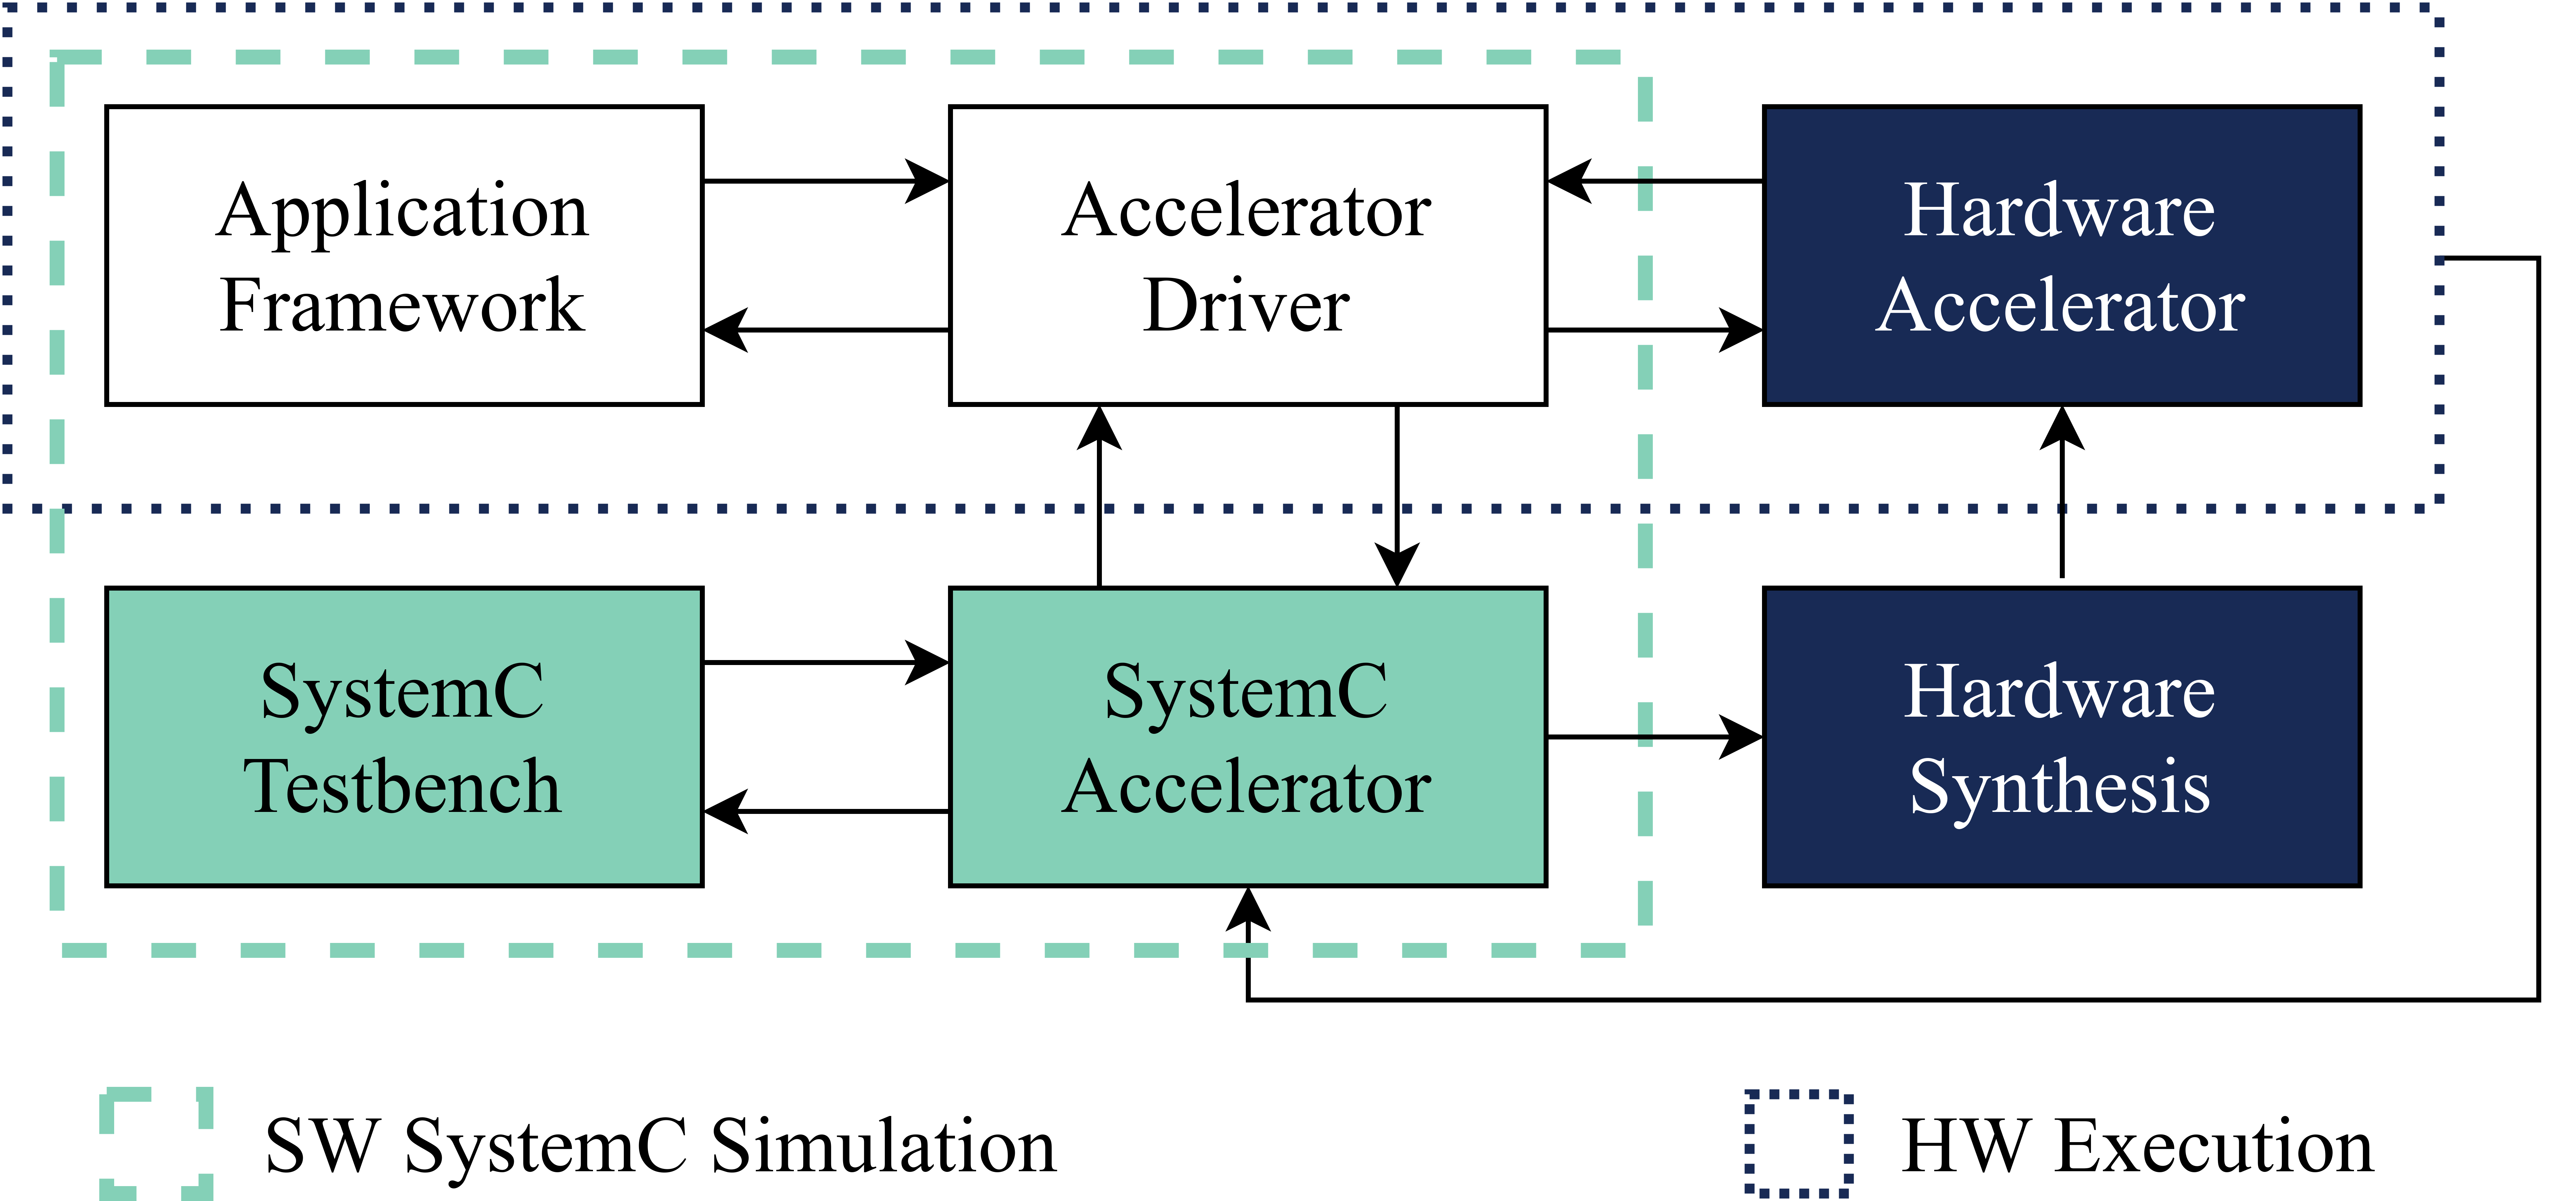
\includegraphics[width=0.9\columnwidth]{files/SECDA_meth.png}
  \caption{\label{fig:secda_method} Overview of the SECDA methodology~\cite{harisSECDAEfficientHardware2021}.
  Components in the dashed lines correspond to simulation, and in the dotted lines to execution on real hardware.}
\end{figure}


As such, we aimed to employ SECDA (SystemC Enabled Co-design of DNN Accelerators)~\ref{fig:secda_method}, a hardware-software design methodology to efficiently produce optimized inference accelerators for edge devices using FPGAs.
SECDA uses SystemC~\cite{IEEE2012systemc} as an accelerator simulation framework, allowing candidate designs to be efficiently iterated upon.
Additionally, SECDA uses SystemC High-Level Synthesis (HLS) to produce a synthesizable design based on the same SystemC accelerator definition.
One key aspect of SECDA is the full integration of the design process with the target application framework.
For LLMs inference, \LPP is the ideal target application framework.
With the integration of \LPP as the application framework, it becomes feasible to convert an LLM to the GGUF format and execute LLMs on edge FPGA-based platforms.



% like ZYNQ~\cite{zynq} is possible.


% Subsequently, within the SECDA-LLM platform, executing the GGUF format model on FPGA-based SoCs like Zynq is possible.
% Profiling the model with our SECDA tools allows us to understand the bottlenecks of the model.
% Following the bottleneck analysis, leveraging SECDA-LLM, designing an accelerator tailored for a specific part of the model is possible.
% Once the accelerator design is finalized, designers can offload designated tasks to the FPGA accelerator while the LLM model continues to run on the CPU.



% Design process

% We attempted to identify FPGA-based accelerator design process for LLMs.
% \cite{Lu2020Transformer} proposed a transformer accelerator design that commences with the C/C++ code of an LLM model.
% While their primary focus lies on the accelerator design aspect, they do not necessarily emphasize the design process itself.


 % FPGAs possess the capability to prototype acceleration ideas that can be beneficial for both quantization types and layer types.

% LLM -> GGUF -> compressed , quantised floats -> execution decompression of weights and float VEC\_DOT
% weight are quantised/compressed and inputs are not
